% Created 2018-04-28 Sat 22:14
\documentclass[11pt]{article}
\usepackage[utf8]{inputenc}
\usepackage[T1]{fontenc}
\usepackage{fixltx2e}
\usepackage{graphicx}
\usepackage{longtable}
\usepackage{float}
\usepackage{wrapfig}
\usepackage{rotating}
\usepackage[normalem]{ulem}
\usepackage{amsmath}
\usepackage{textcomp}
\usepackage{marvosym}
\usepackage{wasysym}
\usepackage{amssymb}
\usepackage{hyperref}
\tolerance=1000
\usepackage{hyperref}
\usepackage{cleveref}
\usepackage{xcolor}
\usepackage{amsmath}
\hypersetup{colorlinks=true}
\author{Zhao Wei}
\date{\today}
\title{COSC420 Neural Network Assignment Report}
\hypersetup{
  pdfkeywords={},
  pdfsubject={},
  pdfcreator={Emacs 25.3.1 (Org mode 8.2.10)}}
\begin{document}

\maketitle
\tableofcontents


\section{Introduction}
\label{sec-1}
My neural network is a simple fully connected feedforward network with just one hidden layers. The number of input, hidden and output units can be specified through a param.txt file. It reads input pattern and teaching input pattern from input.txt and teaching$_{\text{input}}$.txt respectively. 

This report describes the implementation of my neural network and some tests which uses the dataset from several datasets. 
\section{Background}
\label{sec-2}
My neural network is a fully connected. It implements the general delta rule for backpropagation and uses sigmoid function as activation function. During initialization, if the number of patterns in data is 150(which is iris flow dataset), then it raondomly select 100 patterns as training dataset, the rest 50 patterns will be used as testing dataset. If the dataset is very simple one, it will not devide dataset into training and testing, since the dataset is so small, and we need every pattern in it to train. My training uses the online approache. It means the backpropagation will be done for every input pattern. Also I shuffle the dataset before every epoch.

Since the main structure of the network is mearly fixed. My experiments focus on the changes of learning rate, number of hidden units and using testing accuracy as learning criteria.

\section{Experiment}
\label{sec-3}
\subsection{Change the learning rate}
\label{sec-3-1}
Learning rate plays an important role, since it appears in almost every machine learning algorithm. How to set it is based on some heuristic, so I want to see the effect of it on my neural network. I use the iris dataset, and collect training epochs while changing the learning rate with different value.

Table \ref{table-epochs-needed} shows the epochs needed to train my neural network to \texttt{learning\_criteria (popErr) = 0.05} with different learning rate on iris dataset. Other parameters are the same including learning momentum is 0.9.

\begin{table}[htb]
\caption{table shows the epochs needed to reach a popErr criteria, with different learning rate.  \label{table-epochs-needed}}
\centering
\begin{tabular}{rrrrrrr}
id & r=0.2 & r=0.15 & r=0.13 & r=0.11 & r=0.08 & r=0.05\\
\hline
1 & 66 & 55 & 117 & 5705 & 229 & 4441\\
2 & 183 & 301 & N/A & 1571 & 864 & 2375\\
3 & 179 & 216 & 178 & 228 & 310 & 1463\\
4 & 217 & 105 & 205 & N/A & 259 & 7884\\
5 & 513 & 135 & 1922 & 237 & 898 & 379\\
6 & 92 & N/A & 169 & 1791 & 3015 & 1124\\
7 & N/A & 172 & 755 & 2318 & N/A & 1111\\
8 & 6748 & 170 & 124 & 226 & 1851 & 269\\
9 & 842 & 338 & 313 & N/A & 2429 & N/A\\
10 & 75 & 155 & 7656 & 566 & 463 & 309\\
11 & 49 & 466 & N/A & 193 & 258 & 383\\
12 & 68 & 2233 & 123 & N/A & 121 & 719\\
13 & 344 & 1872 & 176 & 608 & 167 & 621\\
14 & 43 & 80 & 289 & 98 & 388 & 250\\
15 & 81 & 6862 & 5623 & 128 & 255 & 325\\
16 & 128 & 69 & 179 & 234 & 214 & N/A\\
17 & N/A & 80 & 1077 & 8795 & 831 & 298\\
18 & 3805 & 211 & 262 & 241 & 1386 & 273\\
19 & 3100 & 186 & 110 & 192 & 949 & 617\\
20 & 52 & N/A & 119 & 2885 & 365 & 341\\
21 & 151 & 87 & 483 & 152 & 596 & 1590\\
22 & 3956 & 37137 & 308 & 197 & 223 & 387\\
23 & 48 & 104 & 18465 & 232 & N/A & 1314\\
24 & 83 & 123 & N/A & 122 & 12753 & 279\\
25 & 3100 & 587 & 38938 & N/A & 489 & 171\\
26 & 310 & 130 & 181 & 697 & 479 & 676\\
27 & 151 & 201 & 241 & 150 & 14169 & 6996\\
28 & 204 & 212 & 543 & 243 & 1258 & 19315\\
29 & 703 & 128 & 726 & 148 & 847 & 731\\
30 & 16186 & 3912 & 321 & 241 & 565 & 2763\\
31 & 185 & 182 & 430 & 199 & 2098 & 2420\\
32 & 125 & 312 & 262 & 346 & N/A & 3022\\
33 & 304 & 403 & 647 & 515 & 580 & N/A\\
34 & 61 & 539 & 102 & 798 & N/A & N/A\\
35 & 104 & N/A & 172 & 183 & 236 & 1562\\
\hline
Times of N/A & 2 & 3 & 3 & 4 & 4 & 4\\
Mean & 663.138 & 371.077 & 608.769 & 436.522 & 715.391 & 1078.652\\
\end{tabular}
\end{table}

\begin{itemize}
\item Because sometimes it shows no signs to reach the learning criteria, I have to cancel the training. And the corresponding cell in the table has recorded as N/A.
\item To collect the statistics, I get rid of corresponding number of N/A for minimum and maximum epochs in the each column. For example, there are 2 N/A for r=0.2, so when I compute the average epochs, I will not consider the two smallest and two maximum epochs in r=0.2 column.
\item The final average value is filled in the final row. If we plot it out, it is show in figure \ref{fig-average-epochs}. It shows the general average epochs is increase while decreasing the learning rate.
\begin{figure}[htb]
\centering
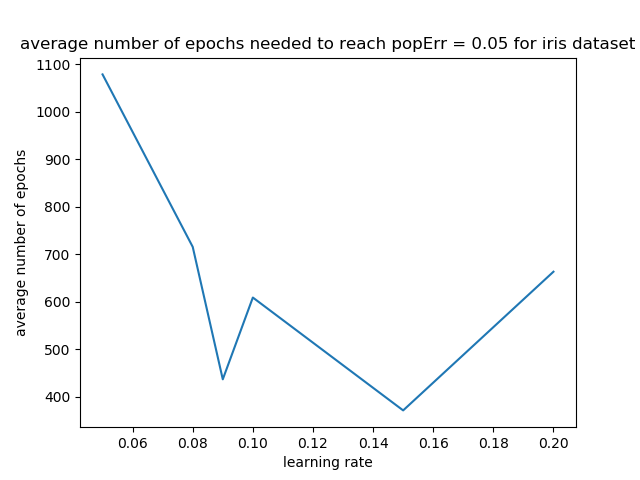
\includegraphics[width=.9\linewidth]{./average_epochs.png}
\caption{shows average epochs needed to reach popErr = 0.05 for training on iris dataset with 6 hidden units \label{fig-average-epochs}}
\end{figure}
\end{itemize}


\subsubsection{Using testing accuracy as criteria}
\label{sec-3-1-1}
Though dozens of experiments, I found out the popErr sometimes could not represent the real effect of learning. After all, we need to generalize well on the training set to confirm the neural network is working which is evaluated by the testing accuracy.  

So, using popErr as learning criteria is not sufficient. Furthermore, a small changes on the popErr could result a big accuracy improvement or even sometimes, the high accuracy does not appear at the lowest popErr, see figure \ref{fig-iris-low-poperr-high-accuracy}.
\begin{figure}[htb]
\centering
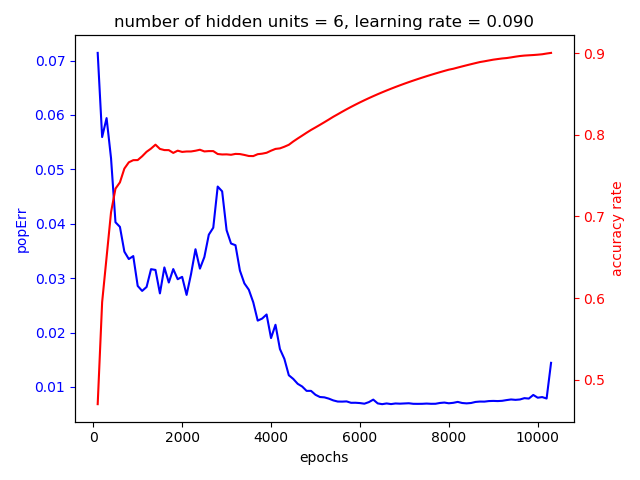
\includegraphics[width=.9\linewidth]{./popErr_vs_accuracy_on_iris_oscillate02.png}
\caption{training on iris dataset, shows lower popErr does not perfectly match high accuracy \label{fig-iris-low-poperr-high-accuracy}}
\end{figure}

Before collecting the testing accuracy, I need to define what is True or False for my learning output. Because the teaching input is integer vector which is used to define classes, there will always some differences between my NN's output and the ground truth. So I define a fit criteria = 0.4, it means if the corresponding attribute between teaching input and NN's out is greater than 0.4, I consider the output is False. For example, during testing I randomly pick a pattern and compare the corresponding attribute difference:
\begin{verbatim}
the input is: [0.137 0.584 0.102 0.043]
the teaching input is: [1. 0. 0.]
the output is: [0.84735159 0.45242708 0.00200901]
the differences between corresponding attribute is > 0.45, so decide it is False.
\end{verbatim}

This simple scheme will help me to compare the proportion of each attribute to decide if it is a correct classification. The reason this works because in the teaching input, there is only 1 attribute will be marked as 1 and the rest is 0.

The accuracy is computed by (the number of True) / (the number of total tested patters). In my program, I will randomly select 100 patterns from testing set. By using testing accuracy as the learning criteria, it alleviates the problem of adjusting the small popErr.

\subsection{Change the number of hidden units}
\label{sec-3-2}
Though experiment, I can feel that the number of hidden units indeed plays the key role. It controls the ability of abstracting the patters from environment.
\subsubsection{Change the number of hidden units for encoder/decoder dataset}
\label{sec-3-2-1}
When I first use default setting to train encoder/decoder dataset (8:3:8), the popErr is aproaching to 0.095 and accurary is around 0.125. That means my neural network is almost not learning.

However, When I increase the number of hidden units to 8. The popErr and accuracy can be improved to a satisfactory level ,see figure \ref{fig-coder-8hidden}.

\begin{figure}[htb]
\centering
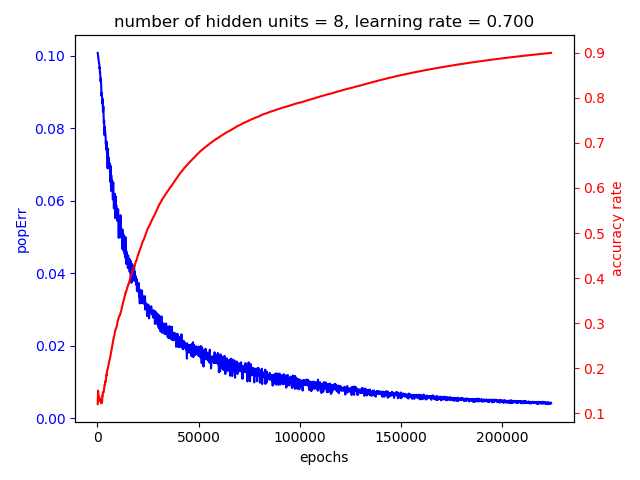
\includegraphics[width=.9\linewidth]{./popErr_vs_accuracy_on_coder.png}
\caption{learning result on the encoder/decoder dataset \label{fig-coder-8hidden}}
\end{figure}


\subsubsection{Change the number of hidden units for iris dataset}
\label{sec-3-2-2}
It is same for iris dataset. When I increases the number of hidden units, it becomes easier to gain a better accurary and lower popErr.
\begin{itemize}
\item For using default 3 hidden units, the training is very slow. I could get a small popErr, but it is not enough to get a high accuracy. The accuracy is around 0.53 \textasciitilde{} 0.67 and could not be improved during training.
\item For using 6 hidden units, the training could be much faster to reach the testing accuracy
\begin{figure}[htb]
\centering
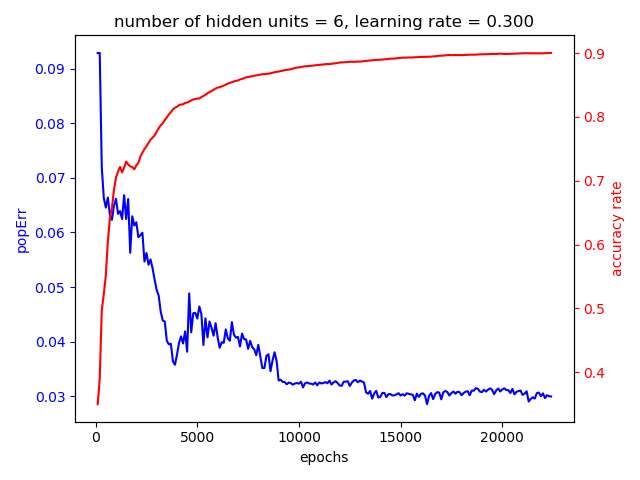
\includegraphics[width=.9\linewidth]{./popErr_vs_accuracy_on_iris_6hidden_0.3r.png}
\caption{training on iris dataset, with 6 hidden units, learning rate = 0.3 \label{fig-iris-6hidden-larger-learning-rate}}
\end{figure}
\item In some cases, even small learning rate can train quickly to get good accuracy, see figure \ref{fig-iris-6hidden-quick-learn}.
\begin{figure}[htb]
\centering
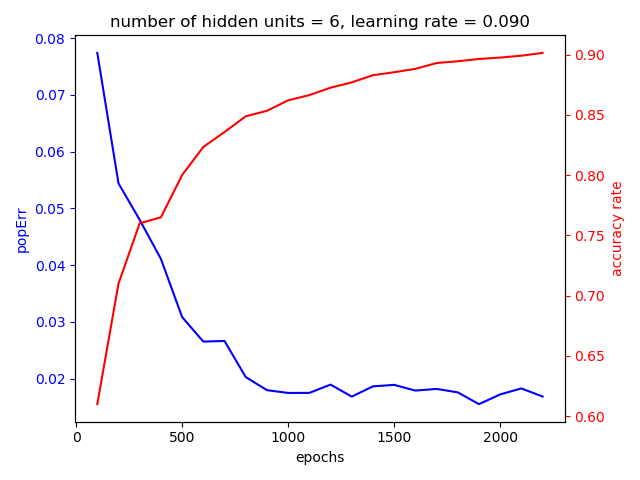
\includegraphics[width=.9\linewidth]{./popErr_vs_accuracy_on_iris_very_quickly.png}
\caption{sometimes the network could be trained very quickly using a small learning rate \label{fig-iris-6hidden-quick-learn}}
\end{figure}
\end{itemize}

\section{Discussion}
\label{sec-4}
Though the experiments on training my neural network, I notice several points:
\begin{enumerate}
\item Larger learning rate can reduce popErr faster than smaller learning rate.
\item However, popErr is hard to used a learning criteria, so I defined the testing accuracy criteria. And find out smaller learning rate can usually reach high accuracy. The reason is to get a high accuracy, the popErr need to be reduced to a smaller value, but big learning rate make the neural network oscillate on the error surface and could not settle down to the minimum.
\item Increase the number of hidden units could boost the learning capacity of neural network. Though my experiments it is clear to see that without the extra number of hidden units a high accuracy could not be reached.
\item The initial state of neural network is very important. Sometimes, same settings with different initial weights will behave very differently. For example, the epochs needed to train neural network to a high accuracy with same settings could be very different, see table \ref{table-epochs-variance-on-iris}.
\end{enumerate}
\begin{table}[htb]
\caption{table shows the big variance of training epochs of training to accuracy = 0.9 on iris dataset with 6 hidden units \label{table-epochs-variance-on-iris}}
\centering
\begin{tabular}{rr}
id & learning rate = 0.09\\
\hline
1 & 1000\\
2 & 900\\
3 & 2800\\
4 & 22100\\
5 & 300\\
6 & 2000\\
7 & 1400\\
8 & 10300\\
9 & 1500\\
10 & 1400\\
\hline
\end{tabular}
\end{table}

In general, it is useful to define different kinds of method to guid the network training, to reach a result you expected. But it is hard to speicify a uniform rule so that as long as you follow that you could reach the goal. Moreover, if the training of neural network is like walking on the error surpace to reach the global lowest place, then whether you could reach there not only depend on the method you used, but also depends on the initial place you start. That is very hard to control. That's why there is big variance on my training epochs.

\section{Appendix}
\label{sec-5}
The whole program is implemented with Python. It uses Numpy for dataset manipulation.
\subsection{The component of the program}
\label{sec-5-1}
\begin{itemize}
\item NeuralNetwork.py, is the model which contains the class NN for abstract a fully connected neural network.
\item main.py, is the controller. It contains the main entry point to call NN's different method based on user's input.
\item It also contains three .txt file for storing the information about parameters, input, and teaching input respectively.
\end{itemize}
\subsection{Usage}
\label{sec-5-2}
\subsubsection{How to run the program}
\label{sec-5-2-1}
Run \texttt{python ./main} on commmand-line.
The program will try to load 3 files in the same directory: param.txt, input.txt and teaching$_{\text{input}}$.txt. You could also changes the corresponding part within code:
\begin{verbatim}
def initialize(self):
    params = np.loadtxt('param.txt')
    inputs = np.loadtxt('input.txt')
    teachingInput = np.loadtxt('teaching_input.txt')
\end{verbatim}
\subsubsection{How to use the program}
\label{sec-5-2-2}
When It runs, it will goes into a loop to wait the user's input:
\begin{verbatim}
Please input 0 - 9 to select:
1 : initialize
2 : teach 100 epochs
3 : teach until accuracy >= 0.90 during testing
4 : teach to criteria
5 : randomly select one patter to test
6 : show weights
7 : run 100 test and collect training result
8 : check hidden units
9 : check settings without re-initialize the net
0 : quit
your choice =>
\end{verbatim}

\begin{itemize}
\item You need to first initialize the neural network
\item Then, you could chose other options. Notice, the option 3 and 4 will keep training the neural network until it reaches the pre-specific settings.
\item If you want to start another training, you could restart the program or choose option 1 to reset the whole program to initial state.
\item Option 8 is used to check the hidden units state, it is usefult for testing the training result on encoder/decoder dataset which the hidden units are learning the code book.
\end{itemize}
% Emacs 25.3.1 (Org mode 8.2.10)
\end{document}